%  !TeX  root  =  user_guide.tex 

\section{Plugin Cattura coordinate}\label{coordcapt}

% when the revision of a section has been finalized, 
% comment out the following line:
% \updatedisclaimer

Il plugin Cattura Coordinate permette di mostrare sulla mappa coordinate in due sistemi di riferimento distinti.

\begin{figure}[ht]
   \centering
   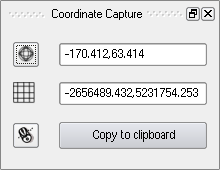
\includegraphics[clip=true, width=8cm]{coordinate_capture_dialog}
   \caption{Plugin Cattura coordinate \nixcaption}\label{fig:coordinate_capture_dialog}
\end{figure}


\begin{enumerate}
  \item Avviare QGIS, aprire le proprietà del progetto \dropmenuopttwo{mActionOptions}{Proprietà Progetto...} nel menu
  \mainmenuopt{Impostazioni} (KDE, Windows) o \mainmenuopt{File} (Gnome, OSX) e scegliere la 
  scheda \tab{Sistema di riferimento (SR)}. In alternativa, cliccare sull'icona 
  \toolbtntwo{mIconProjectionEnabled}{Stato SR} nell'angolo in basso a destra della barra di stato.
  \item Attivare \checkbox{Abilita la riproiezione al volo} e selezionare un sistema di coordinate
  proiettate a scelta (Sezione \ref{label_projections}).
  \item Attivare il plugin Cattura Coordinate nel Gestore dei plugins (Sezione \ref{sec:load_core_plugin}) 
  ed assicurarsi che il dialogo sia visibile verificando che \checkbox{Cattura coordinate}, in 
  \mainmenuopt{Visualizza} > \dropmenuopt{Pannelli}, sia selezionato. 
  La finestra di dialogo Cattura coordinate è mostrata in Figura \ref{fig:coordinate_capture_dialog}.
  \item Cliccare su \toolbtntwo{geographic}{Clicca per selezionare il SR da usare durante 
  la visualizzazione delle coordinate} e selezionare un SR diverso da quello selezionato precedentemente.
  \item Cliccare su \button{Start capture} per iniziare la cattura delle coordinate. Cliccare un punto nella mappa 
  e il plugin mostrerà le coordinate espresse nei due SR selezionati.
  \item Per abilitare la tracciatura via mouse delle coordinate selezionare l'icona \toolbtntwo{tracking}{Clicca per abilitare la tracciatura mouse...}.
  \item Le coordinate selezionate possono essere copiate negli appunti.
\end{enumerate}

\FloatBarrier